\documentclass[12pt]{article}

\usepackage{answers}
\usepackage{setspace}
\usepackage{graphicx}
\usepackage{enumitem}
\usepackage{multicol}
\usepackage{mathrsfs}
\usepackage[margin=1in]{geometry} 
\usepackage{amsmath,amsthm,amssymb}
 
\newcommand{\N}{\mathbb{N}}
\newcommand{\Z}{\mathbb{Z}}
\newcommand{\C}{\mathbb{C}}
\newcommand{\R}{\mathbb{R}}

\DeclareMathOperator{\sech}{sech}
\DeclareMathOperator{\csch}{csch}
 
\newenvironment{theorem}[2][Theorem]{\begin{trivlist}
\item[\hskip \labelsep {\bfseries #1}\hskip \labelsep {\bfseries #2.}]}{\end{trivlist}}
\newenvironment{definition}[2][Definition]{\begin{trivlist}
\item[\hskip \labelsep {\bfseries #1}\hskip \labelsep {\bfseries #2.}]}{\end{trivlist}}
\newenvironment{proposition}[2][Proposition]{\begin{trivlist}
\item[\hskip \labelsep {\bfseries #1}\hskip \labelsep {\bfseries #2.}]}{\end{trivlist}}
\newenvironment{lemma}[2][Lemma]{\begin{trivlist}
\item[\hskip \labelsep {\bfseries #1}\hskip \labelsep {\bfseries #2.}]}{\end{trivlist}}
\newenvironment{exercise}[2][Exercise]{\begin{trivlist}
\item[\hskip \labelsep {\bfseries #1}\hskip \labelsep {\bfseries #2.}]}{\end{trivlist}}
\newenvironment{solution}[2][Solution]{\begin{trivlist}
\item[\hskip \labelsep {\bfseries #1}]}{\end{trivlist}}
\newenvironment{problem}[2][Problem]{\begin{trivlist}
\item[\hskip \labelsep {\bfseries #1}\hskip \labelsep {\bfseries #2.}]}{\end{trivlist}}
\newenvironment{question}[2][Question]{\begin{trivlist}
\item[\hskip \labelsep {\bfseries #1}\hskip \labelsep {\bfseries #2.}]}{\end{trivlist}}
\newenvironment{corollary}[2][Corollary]{\begin{trivlist}
\item[\hskip \labelsep {\bfseries #1}\hskip \labelsep {\bfseries #2.}]}{\end{trivlist}}
 
\begin{document}
 
% --------------------------------------------------------------
%                         Start here
% --------------------------------------------------------------
 
\title{Homework 8}%replace with the appropriate homework number
\author{Seongjin Bien, Mohit Shrestha\\ %replace with your name
Machine Learning - Spring 2018} %if necessary, replace with your course title
 
\maketitle
For this assignment, we trained a sequence of different classifiers with increasing model flexibility, with a varying number of feature vectors. For each of our classifiers, we followed the 6-step procedure documented in the homework sheet. The features we chose were all obtained via PCA, extracting the first k columns from the PCA matrix. We varied the linear regression results from k = 1 to k = 240. The results of this can be seen in Figure 1:\\
\begin{center}
	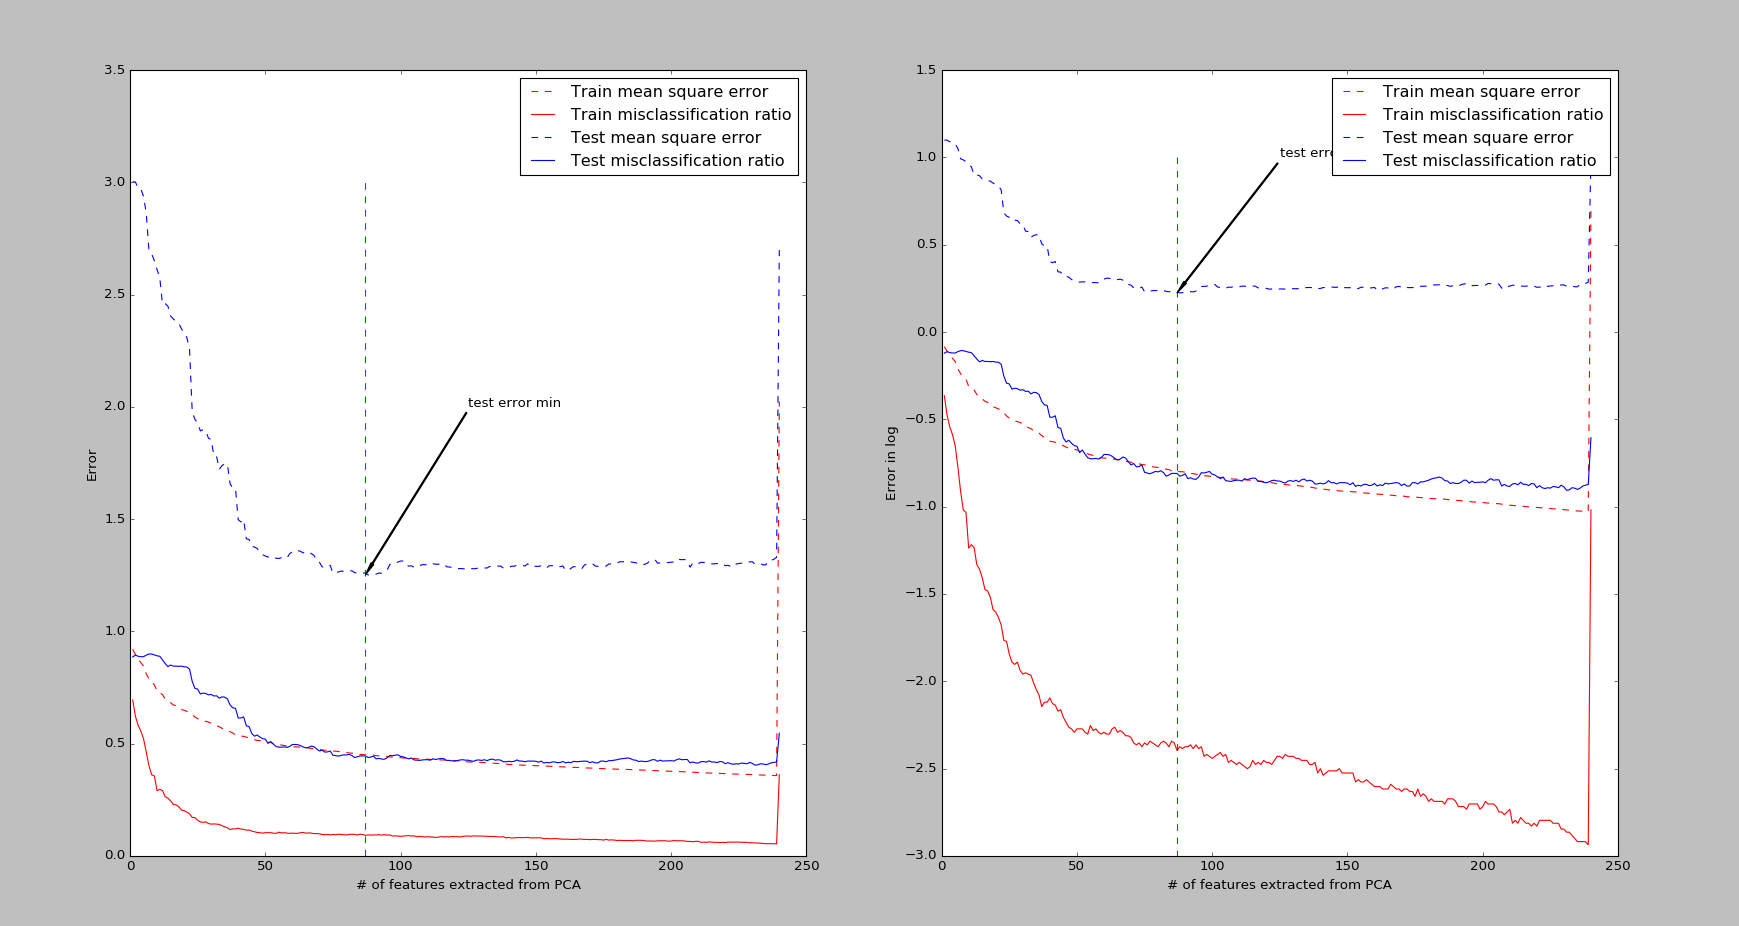
\includegraphics[scale=0.30]{hw8plots.png}\\
	Figure 1. Left: Linear scaling, Right: Logarithmic scaling
\end{center}
    As expected, the $MSE_{Test}, MC_{Test}, MSE_{Train}$ and $MC_{Train}$ all decrease logarithmically with increasing number of features k. Both $MSE_{Train}$ and $MC_{Train}$ decrease as expected with increasing number of k. However, this trend only continues until k = 87, at which the minimum $MSE_{Test}$ is reached. This is more noticeable in the log plot. The value shows a minor increase afterwards, which implies overfitting, but this is not very significant. We assume that this is due to us using PCA and linear regression together, which results in affine linear map from beginning to the end. This results in a less-than-ideal result, as shown here in the miniscule increase in $MSE_{Test}$ and the fact that the convergence rate is much slower than the textbook example of k around 40, meaning more features are needed to reach the same point. $MC_{Test}$ shows a much more inconsistent behaviour and greater jitter, as it was only implicitly targeted by the algorithm. 
\begin{center}
    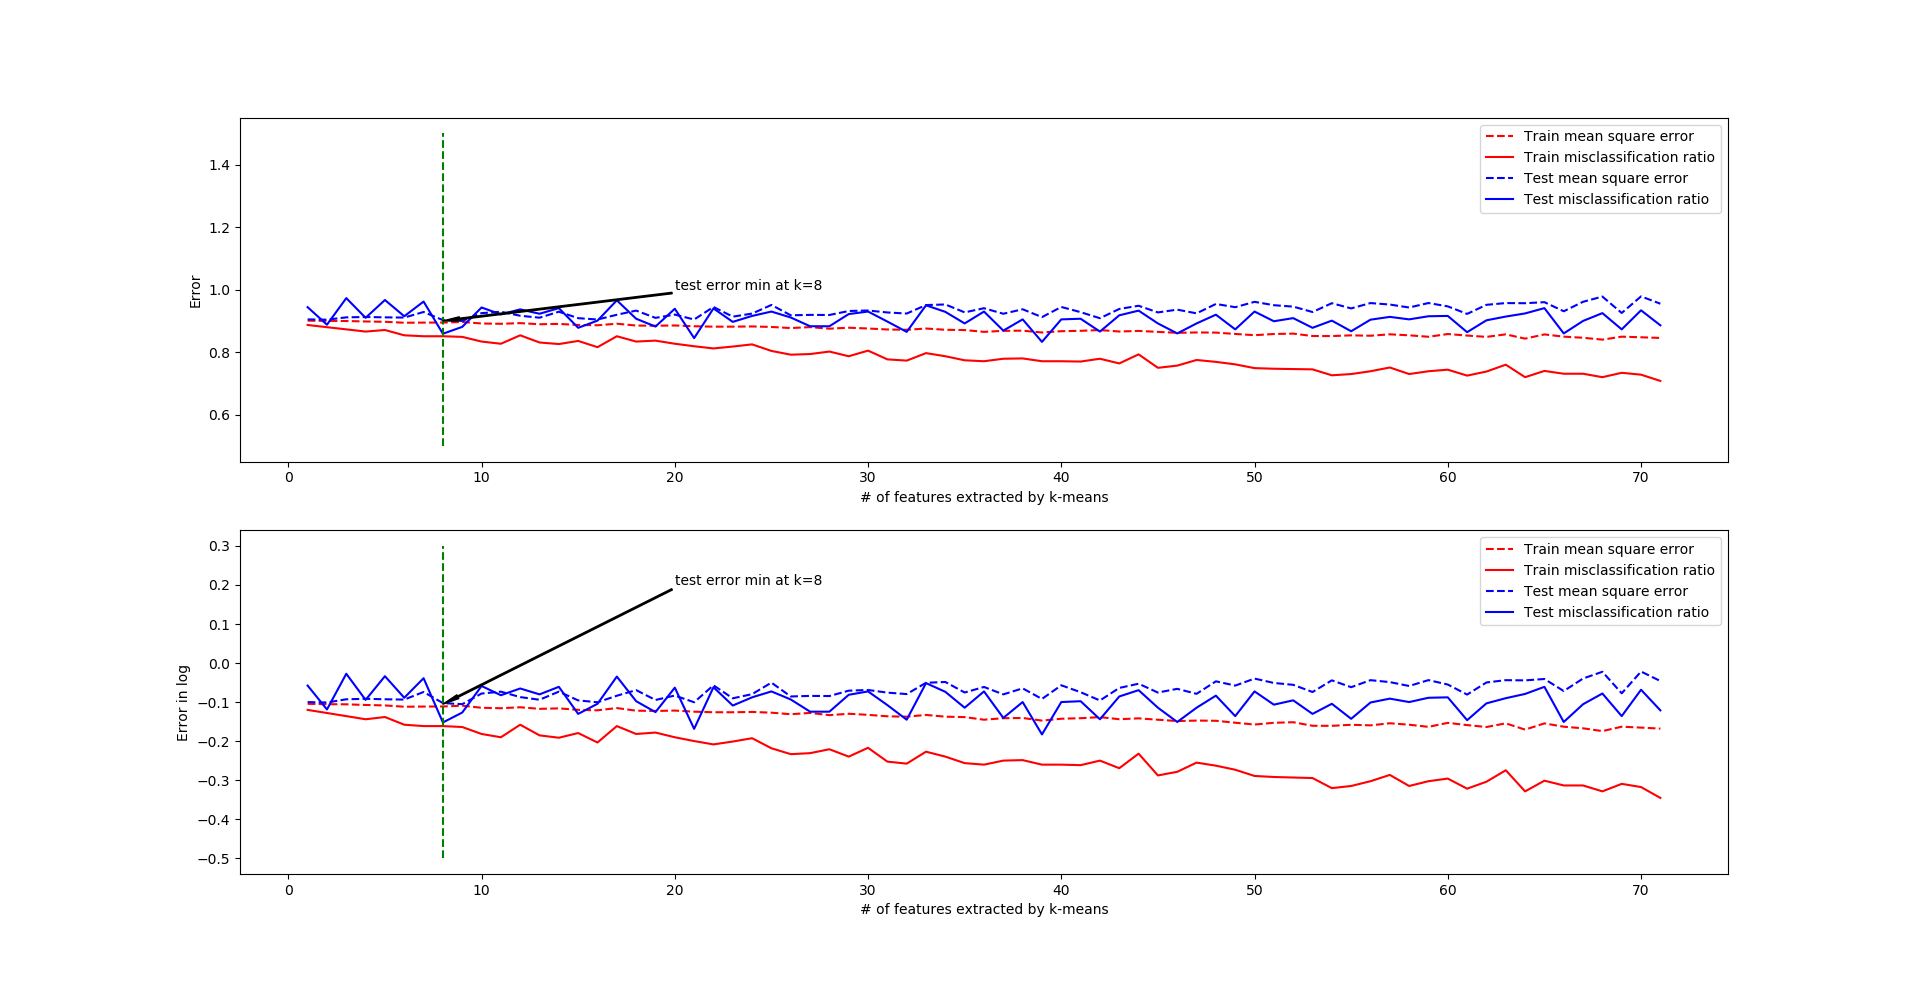
\includegraphics[scale=0.25]{kmeans.png}\\
    Figure 2. Top: Linear scaling, Bottom: Logarithmic scaling    
\end{center}
    The data was pre-processed again, this time with k-means clustering for verifying the above results. As it can be seen in the graph, the minimum $MSE_{Test}$ was reached much more quickly than with PCA at k = 8, after which the data showed overfitting behaviour. Both $MSE_{Train}$ and $MSE_{Test}$ showed continued decrease for increasing number of k after k = 8, which is consistent with our previous analysis with PCA. Unlike the examples in the lecture note, the shape of the plots is much flatter, but the results are still theoretically consistent. We believe the shape and the high jitter are due to the lack of any resampling done on the data, so the results are very rough. The jittering should be reduced if the computation is repeated and and averaged. 
\end{document}
